\chapter[Backward Monte Carlo
Simulation of Atmospheric Muons]{Backward Monte Carlo
Simulation \\of Atmospheric Muons}\label{ch:cosmics}

% \begin{markdown}

% 1. Intro to BMC: relation to adjoint MC (find refs), maybe diagram

% 2. Physics: how we use BMC to determine rates of cosmic events: equations for
% flux, sampling PDF, BMC weights, topography map of J-PARC

% 3. Integration into ICEDUST: implementation of sampling methods, event loop, output to
% oaRooTracker format
% + `https://gitlab.in2p3.fr/comet/ICEDUST_packages/-/merge_requests/534`
% + `https://gitlab.in2p3.fr/comet/ICEDUST_packages/-/wikis/Backward-Monte-Carlo-sampling-with-SimBackwardMC#rate-calculation`

% 3. Actual estimation of background rate in Phase-I, maybe just quoting V's
% result

% ---

% \end{markdown}

% Intro
Cosmic ray-induced events represent a significant part of the expected
backgrounds in the COMET experiment, as discussed in
Section~\ref{sec:backgrounds}. Cosmic rays interact with Earth's atmosphere to
produce secondaries with a wide energy spectrum. Some fraction of these
particles will be able to mimic the conversion signal by entering the COMET
detector system. In this chapter, we discuss how backward Monte Carlo simulation
helps to efficiently estimate the atmospheric background rate.

\section{Backward Monte Carlo simulation}

\subsection{Principle}\label{sec:bmc_principle}
Estimating the rate at which atmospheric muons might produce signal-like events
is computationally expensive through standard Monte Carlo simulation methods.
This is due to the fact that the source of atmospheric muons, i.e.\ the
atmosphere, has a much greater spatial extent than the active detector region.
Hence, most cosmic events generated from an atmospheric source will miss the
detector, thus they will not contribute in the estimation of the background
rate, resulting in wasted computation time.

A backward (or adjoint) Monte Carlo simulation is one where the flow of particle
transport is reversed, i.e.\ events are generated in the sensitive detector
volume and propagated backward in time until they reach the source, as
illustrated in Figure~\ref{fig:bmc_configuration}. This method
was initially used in 1967 to estimate gamma-ray and neutron radiation doses in
nuclear reactors~\cite{doi:10.13182/NSE68-A19235,doi:10.13182/NSE69-A19116}.
More recently, backward MC has also been integrated into Geant4
simulations for dosimetry in space, reversing the
electromagnetic physics of electrons, protons and ions~\cite{DESORGHER2010247}.

In the case of muons, a backward transport method was developed by Niess et
al.~\cite{Niess_Barnoud_Carloganu_Menedeu_2018} in the context of muon
tomography. The software package handling the backward simulation,
PUMAS~\cite{NIESS2022108438}, was later adapted to the COMET experiment in order
to refine estimations of the background rate from cosmic rays.
Appendix~\ref{app:bmc_integration} describes how PUMAS was integrated into the
ICEDUST code base to enable this and future studies of the atmospheric muon
background in COMET.

\begin{figure}
    \centering
    \begin{subfigure}[t]{0.49\textwidth}
        \centering
        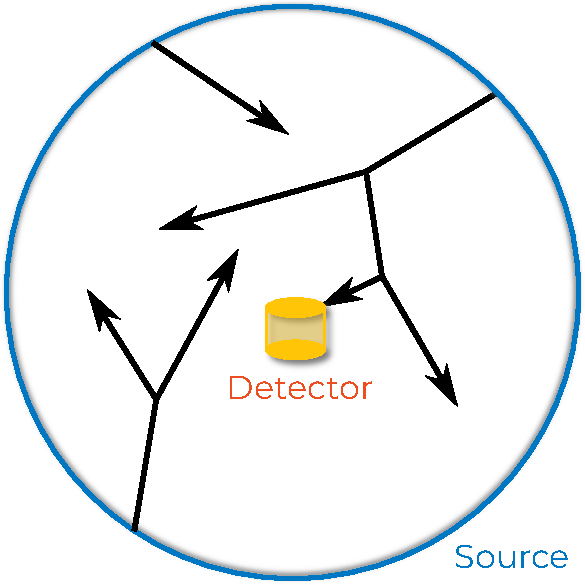
\includegraphics[width=0.66\textwidth]{chapter5/bmc_setup.pdf}
        \caption{Forward MC.}
    \end{subfigure}
    \hfill
    \begin{subfigure}[t]{0.49\textwidth}
        \centering
        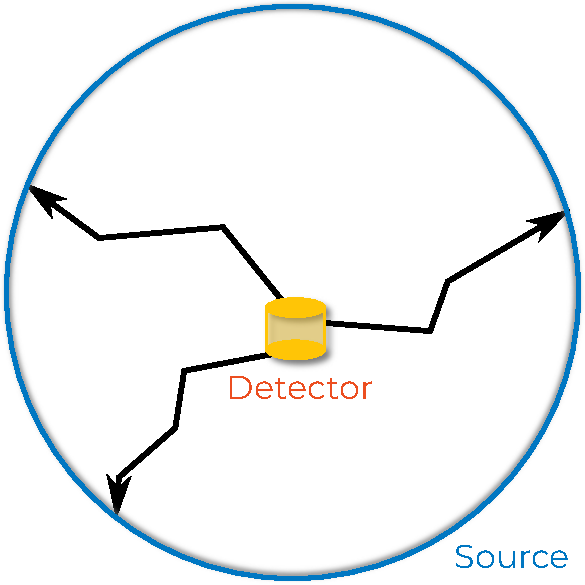
\includegraphics[width=0.66\textwidth]{chapter5/bmc_setup_backward.pdf}
        \caption{Backward MC.}
    \end{subfigure}
    \caption{
        Comparison of the forward and backward (or adjoint) configurations of
        Monte Carlo simulation, in the case where a small detector volume is
        surrounded by a comparatively large particle source. Reversing the flow
        of particle transport means that sampled events are more likely to
        contribute toward the rate estimation.
    }
    \label{fig:bmc_configuration}
\end{figure}

\subsection{Method}
\label{sec:bmc_method}
% In standard Monte Carlo simulations, events are generated by a source and
% propagated forward in time according to their equations of motion and
% interaction cross-sections within any surrounding medium. In a situation where
% the source is large compared to the sensitive detector volume, as illustrated in
% Figure~\ref{fig:bmc_configuration}, events have a high probability to miss the
% % detector and contribute nothing toward the result.

In a backward MC simulation, events are generated according to an arbitrary probability
density function (PDF) around the detector volume. The overall sampling PDF is
typically the composite of a position, direction and energy sampling
distribution, i.e.\ 
\begin{align}\label{eq:sampling_pdf}
p(\bm{x}, \bm{p}, E) = p(\bm{x}) \ \times\  p(\bm{p}) \ \times\  p(E),
\end{align}
where $p$ denotes an arbitrary PDF whose integral is 1, $\bm{x}$ denotes
position, $\bm{p}$ direction and $E$ energy. If more than one particle type is
considered, the discrete distribution of particles can also enter
Equation~\ref{eq:sampling_pdf}. In our case, both atmospheric muons and anti-muons
are relevant, so they are sampled identically and in equal proportions.

\sepfootnotecontent{A}{Reference~\cite{DESORGHER2010247} also provides a more
thorough discussion of adjoint cross-sections, weights, weight corrections and
source normalisation.}

Each event $i$ is propagated backward using adjoint transport and interaction
kernels such that the particle undergoes reverse continuous energy loss and
reverse discrete processes, while moving backward toward the source. At each
step $j$ of the propagation, a multiplicative weight $w^i_j$ is computed given
the path taken and the interactions along it. When the particle reaches the
source, the directional flux at the source $\phi_\mathrm{s}$ is used as a
normalisation factor to yield a weighted event flux
$$
\phi(\bm{x}'_i, \bm{p}'_i, E'_i) = \prod_j w^i_j\ \times\ 
\phi_\mathrm{s}(\bm{x}'_i, \bm{p}'_i, E'_i),
$$
where $\bm{x}'$, $\bm{p}'$ and $E'$ denote respectively the position, direction
and energy of the particle upon reaching the source.

The weighted event flux $\phi$ is related to the event rate $R$ by the
inverse of the sampling PDF of Equation~\ref{eq:sampling_pdf} used to generate
the event initially:
\begin{align*}
R\,(\bm{x}_i, \bm{p}_i, E_i, \bm{x}'_i, \bm{p}'_i, E'_i) = 
    \frac{\phi(\bm{x}'_i, \bm{p}'_i, E'_i)}{p(\bm{x}_i, \bm{p}_i, E_i)}.
\end{align*}
Since the rate depends on the position, direction and energy of the particle at
the source, it is susceptible to variation across backward runs because of the
stochastic aspect of Monte Carlo transport. Hence, backward transport is
repeated $N$ times for each event to find the average rate
\begin{align}\label{eq:avg_rate}
\overline{R}\:(\bm{x}_i, \bm{p}_i, E_i)
    &= \sum_{k=1}^N R\,(\bm{x}_i, \bm{p}_i, E_i, \bm{x}'_k, \bm{p}'_k, E'_k) \nonumber\\
    &= \frac{1}{p(\bm{x}_i, \bm{p}_i, E_i)} \ \times\ \frac{1}{N} \sum_{k=1}^N \phi(\bm{x}'_k, \bm{p}'_k, E'_k),
\end{align}
smearing out the dependence on $\bm{x}'$, $\bm{p}'$ and $E'$. Given a large
enough $N$, i.e.\ a significant enough sample of backward transports, the sum of
weighted fluxes becomes equivalent to an integration over the possible transport paths
and interactions. Reference~\cite{DESORGHER2010247} demonstrates that the
obtained results are consistent with forward Monte Carlo\sepfootnote{A}.



% Desorgher on the matching between forward and backward MC:
%  The Monte Carlo sampling of a big enough number of reverse tracks is
%  equivalent to the integration of the weight W over all independent variable
%  (E1,O1,Sd,x1,E0, ...) summed over all type of reverse reactions, atomic
%  elements, adjoint primaries, and adjoint secondaries. In this integration the
%  cases where more than one reaction and no reaction occur are also considered
%  and only the tracks reaching the external source are accounted for. By this
%  way the same answer is obtained as in the forward case.



% \section{ICEDUST integration}

% - New SimBackwardMC package.

% - PUMAS~\cite{pumas} as an external, with goupil stuff to handle topography,
% geomag field, etc.



\section{Application to COMET Phase-I}
% Here, talk about the COMET setup: 
% + We want to estimate the rate of background events caused by 
%   muons+secondaries hitting the detector
% + Thus, we sample muons+/- around the envelope of the CRV, according to [spell
%   out PDF]
% + We apply backward MC up to an atmospheric muon flux model at altitude X,
%   tabulated from CORSIKA etc.
% + We can first estimate the cosmic muon rate on each surface of the CRV
%   Show plots etc.
% + From the events generated at the CRV envelope, it is also possible to
%   propagate forward to determine which events might produce signal-like
%   tracks.
% + Once this is done, we use the results from backward propagation to estimate
%   rate of background-inducing cosmic muons, qed.
Backward MC simulation was used to estimate the cosmic background rate in COMET
Phase-I. This section describes the simulation setup, validations of the method
using experimental data, and the results of the study.

\subsection{Geometry}
The simulation geometry used in the simulation is shown in
Figure~\ref{fig:bmc_geometry}. In the COMET \mbox{Phase-I} experiment, the cosmic ray
veto (CRV) described in Section~\ref{sec:crv} will enclose the Cylindrical
Detector in order to help identify events caused by atmospheric muons. The CRV
uses a glass resistive plate chamber (GRPC) as the active detector on the
upstream-facing side, and plastic scintillator counters on the other faces. Two
holes are present in the CRV, one in the upstream face and one in the downstream
face. These holes allow atmospheric muons to sneak into the CyDet unnoticed and
potentially produce signal-like tracks, contributing to the background rate.


\begin{figure}
    \centering
    \begin{subfigure}[b]{0.56\textwidth}
        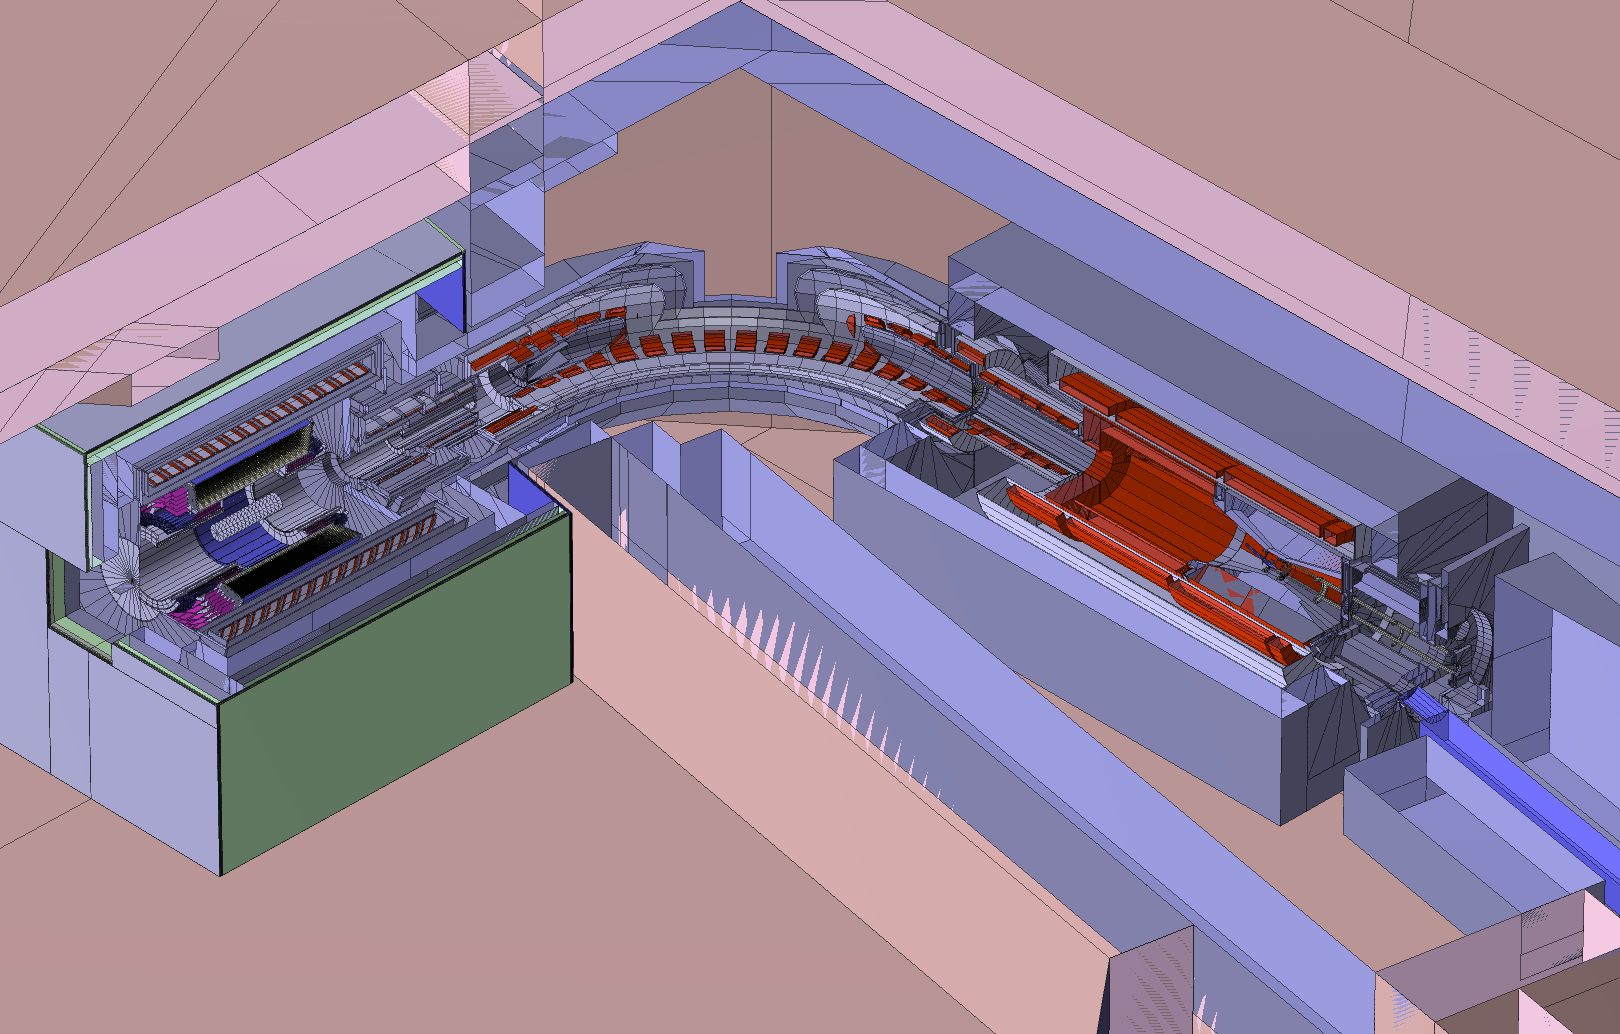
\includegraphics[width=0.95\textwidth]{chapter5/geometry.png}
        \caption{Cutaway view of the simulation world.}
    \end{subfigure}
    \hfill
    \begin{subfigure}[b]{0.41\textwidth}
        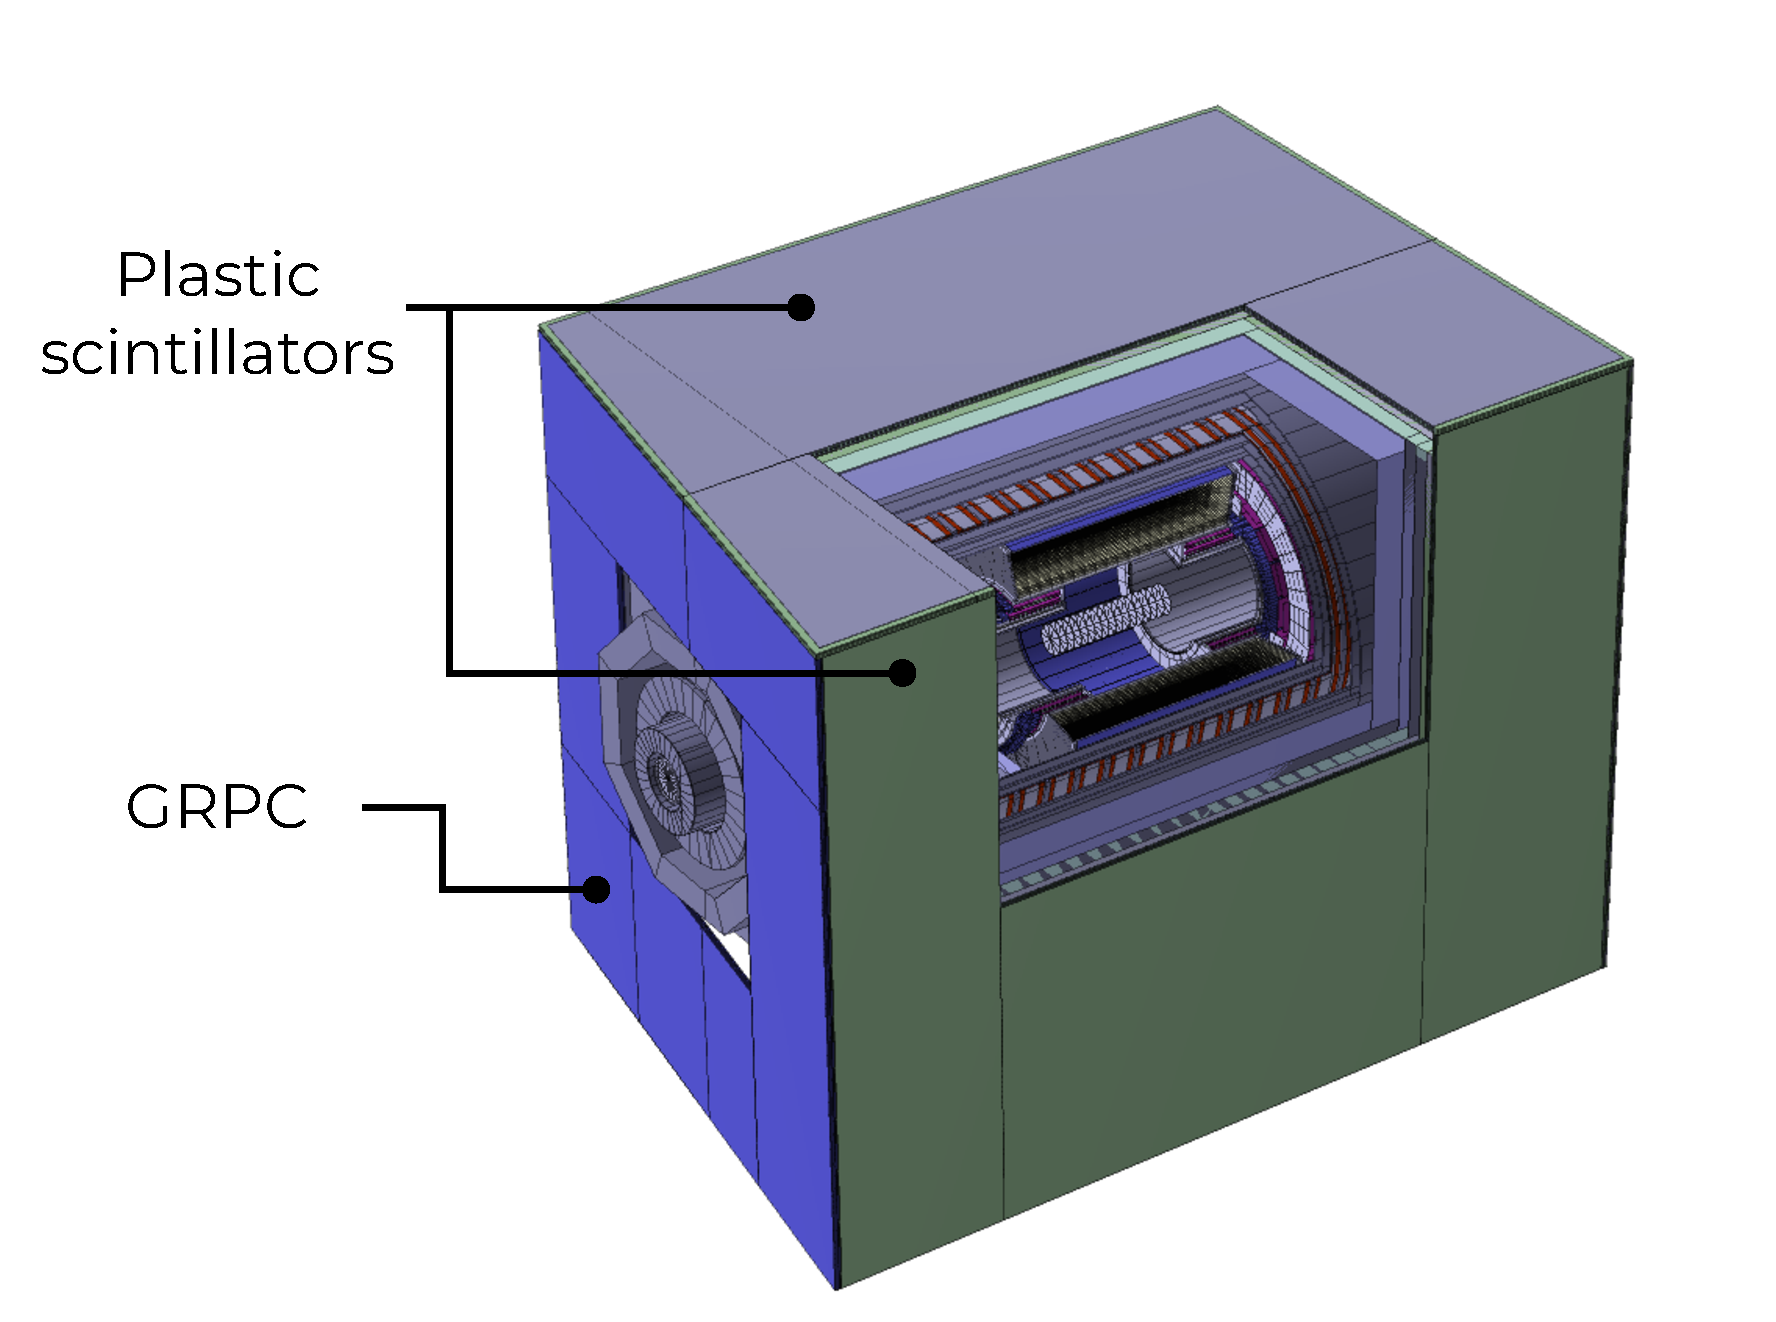
\includegraphics[width=0.95\textwidth]{chapter5/crv_geom.pdf}
        \caption{Detail of the CRV geometry.}
    \end{subfigure}
    \caption{COMET Phase-I simulation geometry used in the cosmic background study.}
    \label{fig:bmc_geometry}
\end{figure}

\subsection{Event sampling}\label{sec:cosmic_event_sampling}

\subsubsection{CRV envelope sample}
As discussed in Section~\ref{sec:bmc_method}, events must be generated around
our volume of interest, the Cylindrical Detector. We define a sampling
envelope around the CRV, where muons (and anti-muons) are generated and
backward-propagated. Events are sampled uniformly over this
envelope, i.e. the position PDF $p(\bm{x})$ is independent of $\bm{x}$:
$$
p(\bm{x}) = \frac{1}{N_{\bm{x}}},
$$
where $N_{\bm{x}}$ is the normalisation term satisfying 
$\int p(\bm{x}) \: \textnormal{d}\bm{x} = 1$.

The direction is sampled according to Lambert's cosine law, which favours events
with a large vertical momentum component:
$$
p(\bm{p}) = 
    \frac{1}{N_{\bm{p}}} \ (-\hat{\bm{p}}) \cdot \hat{\bm{y}} = 
    \frac{1}{N_{\bm{p}}}\:\cos(\theta_z),
$$
where $\theta_z$ is the angle between $-\bm{p}$ and the vertical axis $\hat{\bm{y}}$
(or zenith angle), and $N_{\bm{p}}$ is the normalisation factor. 

The energy is sampled according to an inverse law to
favour low-energy events, since they are more likely on average:
$$
p(E) = \frac{1}{N_E}  \frac{1}{E},
$$
where $N_E$ is the normalisation factor. 

The arbitrary PDFs selected for event sampling do not affect the results so long
as we ensure that no region of the phase-space which could be responsible for
backgrounds is omitted. Here, the direction and energy distributions are
optimised to favour events that are generally more likely to
occur given the configuration of our source and detector (i.e. small zenith
angles and low energies). When computing the rate for an event, any bias
originating from the sampling PDF should be cancelled out when dividing by
$p(\bm{x}, \bm{p}, E)$ as in Equation~\ref{eq:avg_rate}.



\subsubsection{CRV openings sample}
The backward MC method gives freedom to generate a specialised sample to
increase statistics in any region of phase-space. In our case, in order to focus
on the events that might sneak into the detector system, a sample is produced
with events generated only on the holes on either side of the CRV. The energy
and direction are sampled identically to the envelope sample.

Since the position PDF in this sample is concentrated around the holes, we need
to simulate fewer events in order to find a sneaking signal-like track than with
the envelope sample. This allows us to obtain reasonable statistics in the
background rate study while saving on computational resources and storage space.



\subsection{Atmospheric muon flux}
Estimating rates requires knowledge of $\phi_s$, the directional flux at the
source. We use tabulated flux data from a CORSIKA~\cite{corsika} simulation as
an efficient way to query the flux as a function of energy and direction. The
flux data, shown as a function of energy in
Figure~\ref{fig:corsika_flux_distribution}, was estimated \SI{1600}{\metre}
above sea level for energies between \SI{10}{\MeV} and \SI{10}{\TeV}, separately
for muons and anti-muons. In the backward simulation, any event which is unable to
travel back to this infinite source plane is assumed to have a rate of zero.

\begin{figure}
    \centering
    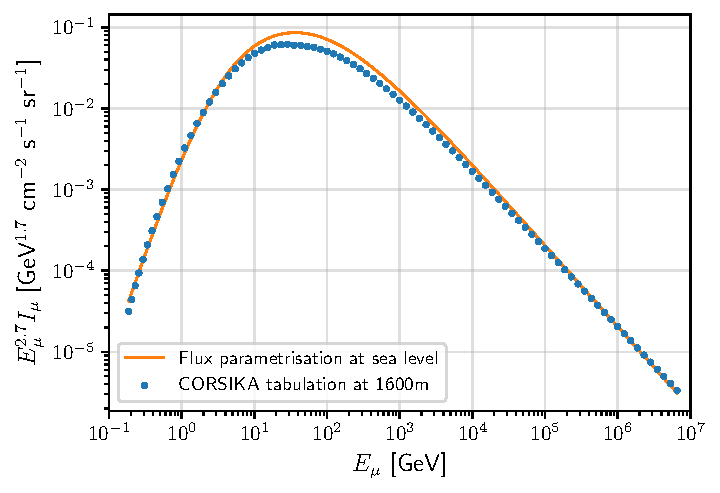
\includegraphics[width=0.6\textwidth]{chapter5/flux_distribution.pdf}
    \caption{ Spectrum of the atmospheric muon flux (multiplied by
        $E_\mu^{2.7}$) calculated at an altitude of 1600m using a CORSIKA
        simulation. This spectrum, tabulated in both energy and zenith angle, is
        used as the flux source in the COMET Phase-I backward MC. Here, it is
        compared with the parametrisation of the muon flux at sea level from Guan
        et al.~\cite{gccly}. }
    \label{fig:corsika_flux_distribution}
\end{figure}

% Do we talk about the PUMAS, GOUPIL setup?
% ICEDUST integration?
% Maybe in appendix

% Describe data sample? How many events generated, how many times
% backward-propagated, how much storage space, etc.

\subsection{Validations}
In order to ensure that the backward MC simulation yields accurate results, the
flux of atmospheric muons estimated around the CRV is compared to two
independent measurements of the flux at sea level.

\subsubsection{BESS-TeV}
The atmospheric muon flux in Manitoba, Canada was measured using the BESS-TeV
spectrometer in 2004~\cite{besstev}. The apparatus only observed muons incident
at an near-vertical zenith angle $\theta_z$. In order to compare our simulation
results with the experimental data, we select simulated events based on the
condition that $\cos \theta_z > 0.98$ to replicate the acceptance of the
spectrometer. The comparison of the differential flux as a function of momentum
is shown in Figure~\ref{fig:bmc_validations_bess}.

\subsubsection{Kiel-DESY}
The Kiel-DESY spectrometer was used to measure the atmospheric muon flux in
Hamburg, Germany in 1975~\cite{kieldesy}. This detector measures particles
within a zenith angle $\theta_z =\SI{75}{\degree} \pm \SI{7}{\degree}$ and an
azimuthal angle $\phi = \SI{288}{\degree} \pm \SI{20}{\degree}$. Similarly to
the previous comparison, simulated events are selected to replicate these
acceptances such that the flux can be compared.
Figure~\ref{fig:bmc_validations_kiel} shows the comparison of the flux spectra.

\begin{figure}
    \centering
    \begin{subfigure}[t]{0.49\textwidth}
        \centering
        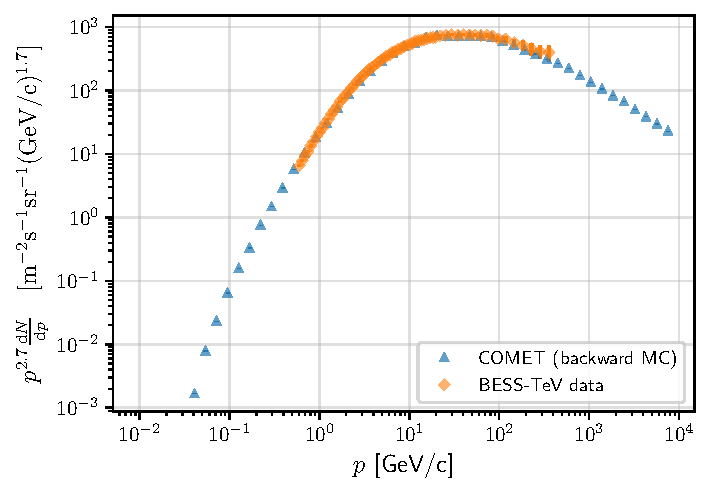
\includegraphics[width=0.95\textwidth]{chapter5/comparison_besstev.pdf}
        \caption{ Comparison to BESS-TeV spectrometer data of the atmospheric
        muon flux at a near-vertical zenith angle in Manitoba,
        Canada~\cite{besstev}. }
        \label{fig:bmc_validations_bess}
    \end{subfigure}
    \hfill
    \begin{subfigure}[t]{0.49\textwidth}
        \centering
        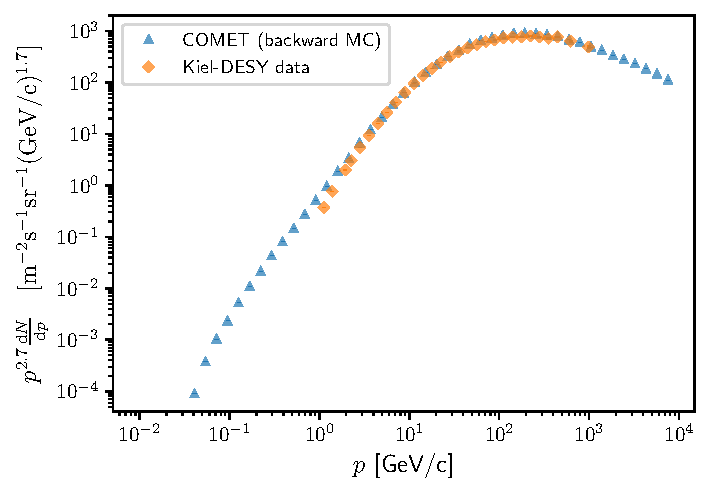
\includegraphics[width=0.95\textwidth]{chapter5/comparison_kieldesy.pdf}
        \caption{ 
            Comparison to the Kiel-DESY spectrometer observation of the
            atmospheric muon flux at a zenith angle of $\SI{75}{\degree} \pm
            \SI{7}{\degree}$~\cite{kieldesy} in Hamburg, Germany.}
        \label{fig:bmc_validations_kiel}
    \end{subfigure}
    \caption{ Validations of the backward MC-estimated flux with experimental
        observations of the atmospheric muon flux by two independent
        experiments. Events from the backward MC simulation are selected to
        reflect the angular acceptance of the corresponding experiment. }
    \label{fig:bmc_validations}
\end{figure}

The fact that both comparisons are in reasonable agreement with the backward
simulation results increases our confidence in the method. Here, we have shown
that the backward MC method can effectively compute the flux of events at sea
level using knowledge of the flux at an altitude of \SI{1600}{\metre}. Note that
our simulation setup differs from either experiment by the amount of material
present between the detector and the atmospheric source. Hence, an imperfect
agreement is expected and the discrepancies visible in either comparison were not
investigated in detail.

\subsection{Absolute rate estimation}
From the estimated flux, one can compute the absolute rate using
Equation~\ref{eq:avg_rate}. Figure~\ref{fig:avg_rate_per_face} shows the
atmospheric muon rate as a function of momentum on each face of the CRV. The top
face is the most exposed, with an integrated rate of \SI{1.97}{\kHz}. Over the
whole surface, the estimated event rate is \SI{3.47}{\kHz}. This estimation of
the rate accounts for all events inbound on the CRV, regardless of whether or
not they enter the CDC or CTH. 


\begin{figure}
    \centering
    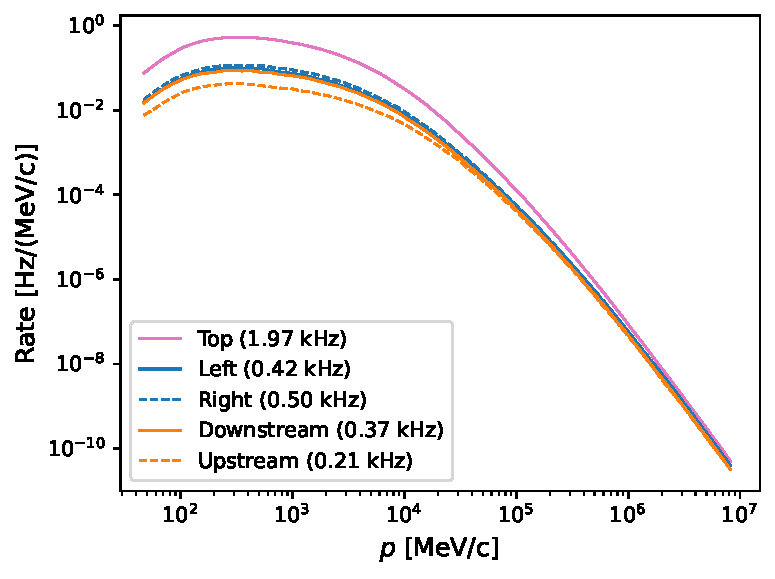
\includegraphics[width=0.5\textwidth]{chapter5/rate_vs_p.pdf}
    \caption{
        Average rate of inbound atmospheric muons over each face of the CRV as a
        function of momentum. Figures in parentheses in the legend are the
        integrated rate averaged over each face.
    }
    \label{fig:avg_rate_per_face}
\end{figure}

\subsection{\texorpdfstring{$\mu$--$e$}{Muon to electron} conversion background
rate}
\label{sec:bmc_conversion_bg_rate}
In order to determine how frequently signal-like tracks are produced by
atmospheric muons, we combine forward and backward MC simulations. The forward
MC allows us to select events based on detector acceptance criteria, such as
trigger conditions. The backward MC is then used to estimate the rate of
selected events.

\subsubsection{Track reconstruction}
After the forward MC step, we also simulate the reconstruction of tracks in the
CDC. The algorithm is a helix fit through the positions of CDC hits. In this step,
the true hit positions given by the \texttt{SimG4} Monte Carlo are used. The fit
also returns the momentum of the reconstructed trajectory, which is used in the
event selection.

% No manual momentum smearing here, since we did helix fit.

\subsubsection{Event selection}
The event selection criteria are as follows:
\begin{itemize}
    \item Fourfold coincidence: four neighbour CTH counters must be hit
    within a \SI{10}{\ns} window,
    \item CDC layers: the track must reach up to the 5th layer of CDC
    wires and no hit should occur on the outermost layer,
    \item Muon stopping target intersection: the fitted track must intersect the
    muon stopping target placed in the centre of the CyDet,
    \item Momentum window: the reconstructed momentum must lie between
    \SI{55}{\MeV/\clight} and \SI{155}{\MeV/\clight}.
\end{itemize}
These criteria reduce the number of events whose flux will be sampled by the
backward MC, which is crucial to limit the usage of computational resources. In
addition, we obtain a reasonably-sized sample from which we can study the shape
and properties of background events.

Other acceptance criteria and inefficiencies of the CyDet system are taken into
account by applying multiplicative factors to the estimated background rates.
Specifically, the hardware efficiency of Table~\ref{tab:acceptance} is used,
reducing the overall background rate by a factor 0.81. To take into account the
fact that the Phase-I trigger is only active during the $t \in [700, 1170]\,
\si{\ns}$ window after each proton pulse, we weight the rate by a factor
$\epsilon_\text{timing} = \frac{8}{9}\,\frac{1170 - 700}{1170} =
\SI{36}{\percent}$, where the term $\frac{8}{9}$ arises from the bunch
structure of the J-PARC main ring.

\subsubsection{Backward sampling}
The flux is sampled by backward MC simulation for all events that pass the above
selection criteria. The backward propagation and flux sampling is performed
$N=5000$ times for each event. The flux for each event is the average over these
$N$ trials, as discussed in Section~\ref{sec:bmc_method}. The variation in the
sampled flux over these $N$ trials is interpreted as the statistical uncertainty
on the average flux for each event. This uncertainty is shown in the resulting
plots and figures.

% \begin{table}[t]
%     \centering
%     \begin{tabular}{l|ccccc}
%         \toprule
%         Criterion&DAQ&Trigger&Track finding&Track quality cuts&Timing window\\\midrule
%         Value&\SI{90}{\percent}&\SI{90}{\percent}&\SI{99}{\percent}&\SI{69}{\percent}&\SI{30}{\percent}\\
%         \bottomrule
%     \end{tabular}
%     \caption{Efficiency factors from the Phase-I
%     TDR~\cite{the_comet_collaboration_comet_2020} applied to obtain the
%     $\mu$--$e$ background rate from atmospheric muons.}
%     \label{tab:bmc_bg_efficiencies}
% \end{table}

\begin{figure}[t]
    \centering
    \begin{subfigure}[t]{0.48\textwidth}
        \centering
        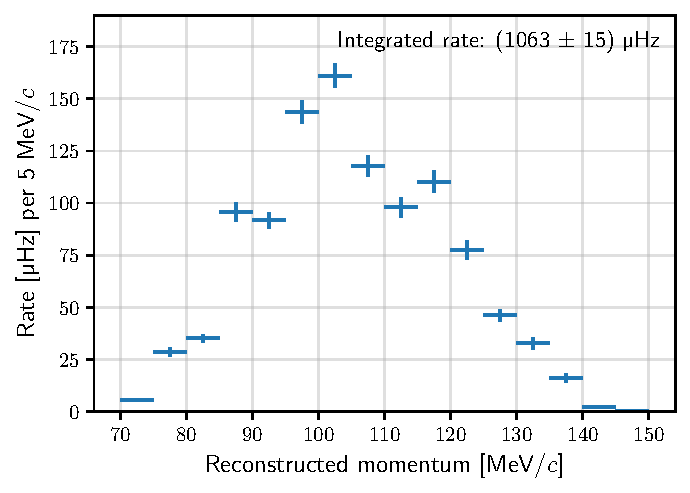
\includegraphics[width=0.99\textwidth]{chapter5/bmc_background_rate_no_crv.pdf}
        \caption{Without a veto.}
        \label{fig:bmc_rate_vs_momentum_no_crv}
    \end{subfigure}
    \hfill
    \begin{subfigure}[t]{0.48\textwidth}
        \centering
        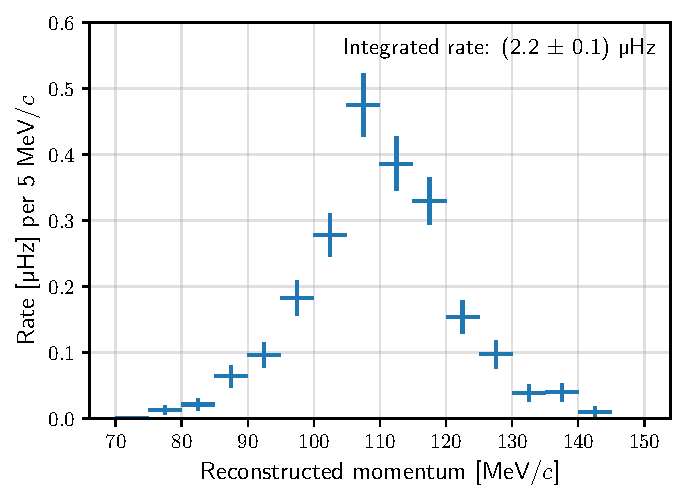
\includegraphics[width=0.99\textwidth]{chapter5/bmc_background_rate_with_crv.pdf}
        \caption{Including the effect of the Cosmic Ray Veto detector, assuming
        an efficiency of \SI{99.99}{\percent}.}
        \label{fig:bmc_rate_vs_momentum_crv}
    \end{subfigure}
    \caption{ 
        $\mu$--$e$ conversion background rates from atmospheric muons
        estimated via backward MC simulation. The error bars show the
        statistical uncertainty on the sampled flux over backward sampling
        trials. In the presence of the CRV, the background rate is dominated by
        events where an atmospheric muon sneaks through the openings. }
        \label{fig:bmc_rate_vs_momentum}
\end{figure}

\subsubsection{Results}
Figure~\ref{fig:bmc_rate_vs_momentum} shows the estimated background rates as a
function of the reconstructed momentum of the signal-like track. We compare the
rate in the absence and in the presence of the CRV to demonstrate its
importance. Without a veto mechanism, the rate over the entire momentum range is
around \SI{1}{\mHz}, and is lowered to \SI{2}{\micro\hertz} with the CRV. The
spectrum peaks around \SI{105}{\MeV}, the conversion energy, because we have
selected events that pass the CTH and CDC trigger criteria. Since the CyDet is
heavily biased toward observing conversion electrons, selected background events
tend to have a signal-like signature.
% Note that in COMET Phase-I, the momentum window
% for the $\mu$--$e$ conversion search is $[103.6, 106.0]$\,\si{\MeV/\clight}. The
% integrated rates shown in Figure~\ref{fig:bmc_rate_vs_momentum} are over the
% entire momentum range of selected events.

In the next chapter, a complete sensitivity and background study for COMET
Phase-I, including the results discussed here, will be presented. Despite the
CRV being expected to reject a large fraction of atmospheric muon backgrounds,
they remain the most important source of backgrounds in the $\mu$--$e$
conversion search. 